\documentclass[a4paper, 12pt]{article}
\usepackage[utf8x]{inputenc}
\usepackage[english, russian]{babel}
\usepackage[left=25mm, top=25mm, right=25mm, bottom=25mm]{geometry}
\usepackage{cmap}
\usepackage{indentfirst}
\usepackage{tikz}
\usepackage{float}
\usepackage{amsmath, amsfonts, amssymb}
\usepackage{graphicx}
\usepackage{hyperref}
\usepackage{listings}
\usepackage{caption}
\usepackage{subcaption}
\usepackage{xcolor}
\usepackage{etoolbox}
\usepackage{titlesec}
\pagestyle{plain}
\patchcmd{\tableofcontents}{\contentsname}{\centering\contentsname}{}{}
\titleformat{\section}[block]{\normalfont\large\bfseries\centering}{}{0pt}{}
\titleformat{\subsection}[block]{\normalfont\normalsize\bfseries\centering}{}{0pt}{}
\allowdisplaybreaks
\graphicspath{{src/images/}}
\usetikzlibrary{patterns}
\definecolor{LightGray}{gray}{0.95}
\definecolor{LightGray2}{gray}{0.7}
\lstdefinestyle{code}{
    language=MATLAB, % replace language here
    basicstyle=\footnotesize\ttfamily,
    % numbers=left,
    % numberstyle=\scriptsize\color{gray},
    % stepnumber=1,
    % numbersep=5pt,
    backgroundcolor=\color{LightGray},
    showspaces=false,
    showstringspaces=false,
    showtabs=false,
    tabsize=4,
    captionpos=b,
    breaklines=true,
    breakatwhitespace=false,
    frame=single,
    rulecolor=\color{LightGray2},
    linewidth=\linewidth,
    keywordstyle=\color{blue}\bfseries,
    commentstyle=\color{green!40!black},
    stringstyle=\color{purple},
    escapeinside={\%*}{*)},
    inputencoding=utf8x,
    xleftmargin=0pt,
    framexleftmargin=0pt,
    framexrightmargin=0pt
}
\lstset{style=code}
\hypersetup{
    colorlinks=true,
    linkcolor=blue,
    filecolor=magenta,
    urlcolor=cyan,
    pdftitle={contents setup},
    pdfpagemode=FullScreen,
}


\begin{document}
    \begin{titlepage}

        \begin{center}
        Федеральное государственное автономное образовательное учреждение высшего образования
        «Национальный Исследовательский Университет ИТМО»
        \vfill
        
        
\includegraphics[width=0.3\textwidth]{itmo.png} % requires /src/images/itmo.png

        {\large\bf ЛАБОРАТОРНАЯ РАБОТА №3}\\
        {\large\bf ПРЕДМЕТ «ТЕОРИЯ АВТОМАТИЧЕСКОГО УПРАВЛЕНИЯ»}\\
        {\large\bf ТЕМА «РЕГУЛЯТОРЫ С ЗАДАННОЙ СТЕПЕНЬЮ УСТОЙЧИВОСТИ»}\\
        Вариант №2
        \vfill

        \begin{flushright}
            \begin{minipage}{.45\textwidth}
            {
                \hbox{Преподаватель:}
                \hbox{Пашенко А. В.}
                \hbox{}
                \hbox{Выполнил:}
                \hbox{Румянцев А. А.}
                \hbox{}
                \hbox{Факультет: СУиР}
                \hbox{Группа: R3341}
                \hbox{Поток: ТАУ R22 бак 1.1.1}
            }
            \end{minipage}
        \end{flushright}
        \vfill
  
        Санкт-Петербург\\
        2025
        \end{center}
    \end{titlepage}
    
    \tableofcontents

    \newpage
    \section{Задание 1. Синтез регулятора с заданной степенью устойчивости}
    Рассмотрим систему
    $$
    \dot{x}=Ax+Bu,\ A=\begin{bmatrix}
        5 &2 &7\\
        2 &1 &2\\
        -2 &-3 &-4
    \end{bmatrix},\ B=\begin{bmatrix}
        3\\1\\-1
    \end{bmatrix};
    $$


    \subsection{Управляемость и стабилизируемость}
    Найдем собственные числа матрицы $A$ и определим управляемость каждого из них. Программа для
    вычислений в \texttt{MATLAB} представлена на листинге \ref{task1code} в приложении 1
    $$
    \sigma\left( A \right)=\left\{-2,2\pm i\right\}
    $$
    Число $\lambda_1=-2$ асимптотически устойчивое, может быть неуправляемым. Комплексная пара $\lambda_{2,3}$
    имеет положительную действительную часть -- эти собственные числа неустойчивые, нужна управляемость.
    Разложим $A$ в вещественную жорданову форму, найдем вектор $B$ в базисе собственных векторов матрицы $A$
    $$
    A=P_{re}J_{re}P_{re}^{-1}=\begin{bmatrix}
    -1    &0.5   &-1.5\\
    0         &0   &-1\\
    1         &0    &1
    \end{bmatrix}\begin{bmatrix}
    -2     &0     &0\\
     0     &2     &1\\
     0    &-1     &2
    \end{bmatrix}\begin{bmatrix}
    0     &1     &1\\
     2    &-1     &2\\
     0    &-1     &0
    \end{bmatrix},
    $$
    $$
    B_{Jre}=P_{re}^{-1}B=\begin{bmatrix}
        0     &1     &1\\
         2    &-1     &2\\
         0    &-1     &0
        \end{bmatrix}\begin{bmatrix}
            3\\
            1\\
            -1
        \end{bmatrix}=\begin{bmatrix}
        0\\
     3\\
    -1
    \end{bmatrix};
    $$
    Итого имеем
    $$
    J_{re}=\begin{bmatrix}
        -2     &0     &0\\
         0     &2     &1\\
         0    &-1     &2
        \end{bmatrix},\ B_{Jre}=\begin{bmatrix}
            0\\
         3\\
        -1
        \end{bmatrix};
    $$
    Все жордановы клетки относятся к различным собственным числам. Только число $\lambda_1=-2$ неуправляемое,
    так как первый элемент $B_{Jre}$ равен нулю. Остальные собственные числа управляемые. Таким образом,
    система не полностью управляема, стабилизируема.


    \subsection{Степень устойчивости}
    Любой степени устойчивости при помощи регулятора $u=Kx$ добиться не получится, так как система не полностью управляема.
    Степень устойчивости системы $\alpha$ -- самое близкое
    к правой комплексной полуплоскости собственное число матрицы $A$,
    находящееся в левой комплексной полуплоскости. Проверка на близость
    осуществляется через действительную часть собственного числа. Имеем
    $$
    \text{Re}\left\{ \lambda_1=-2 \right\}=-2,\ \text{Re}\left\{ \lambda_{2,3}=2\pm i \right\}=2;
    $$
    Таким образом, степень устойчивости системы $\alpha=2$. Это максимум. Устойчивость в данном случае
    подразумевается экспоненциальная.


    \subsection{Схема моделирования системы, замкнутой регулятором}
    Построим схему моделирования системы $\dot{x}=Ax+Bu$, замкнутой регулятором $u=Kx$, используя \texttt{SIMULINK}
    \begin{figure}[H]
        \centering
        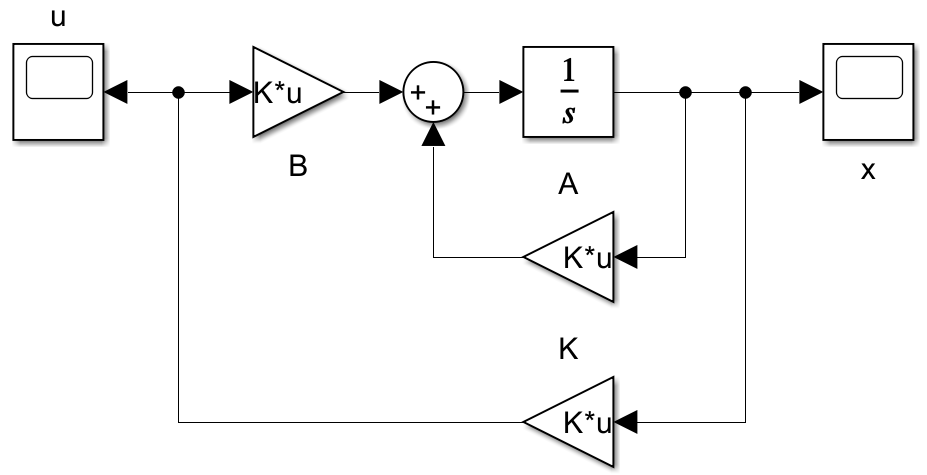
\includegraphics[scale=0.5]{scheme_task1.png}
        \captionsetup{skip=0pt}
        \caption{Схема моделирования системы, замкнутой регулятором}
        \label{fig:scheme_task1}
    \end{figure}


    \subsection{Значения желаемой степени устойчивости}
    Возьмем достаточно отличающиеся достижимые степени устойчивости в диапазоне $0<\alpha\leq2$
    \begin{align*}
        &\alpha_{1}=2\\
        &\alpha_2=0.1
    \end{align*}


    \subsection{Синтез регулятора}
    Для каждого из выбранных значений $\alpha$ синтезируем регулятор, обеспечивающий
    заданную степень устойчивости, при помощи матричного неравенства типа Ляпунова
    $$
    PA^T+AP+2\alpha P+Y^TB^T+BY\preceq0,\ K=YP^{-1}
    $$


    Найдем для $\alpha_{1,2}$ соответствующие матрицы регулятора $K_{1\,\alpha i}$ \textbf{без ограничений на управление}.
    Пользуемся пакетом \texttt{cvx} для \texttt{MATLAB}. Получаем
    $$
    K_{1\,\alpha1}=\begin{bmatrix}
        2.7699  &-19.5247    &1.8232
    \end{bmatrix},\ K_{1\,\alpha2}=\begin{bmatrix}
        -1.9735   &-4.0489   &-2.7179
    \end{bmatrix}
    $$


    Найдем для $\alpha_{1,2}$ соответствующие матрицы регулятора $K_{2\,\alpha i}$ \textbf{совместно с решением задачи минимизации управления}.


    \section{Приложения}
    \subsection{Приложение 1}
    \begin{lstlisting}[label=task1code, caption={Программа для задания 1}]
        to be done
    \end{lstlisting}
\end{document}